% !TEX root = 99_main.tex

For the purposes of this publication, only an initial analysis of the collected environmental quality preference data is provided. The emphasis is to apply an unsupervised clustering technique to the occupant data to segment the users who provide more than five feedback points into cohorts of similar behavior. 

\subsection{Discovering occupant personal comfort preferences}
 
As shown in Figure \ref{fig:clustering}, five distinct clusters can be observed based on differences in preferences for temperature, light and noise levels across users. Predominantly users were comfortable and seldom preferred a change to cooler or quieter environments. Its interesting to discover differences in user "types" based on the clustering. For instance, type \emph{A} prefers quieter spaces as compared to others, whereas \emph{B} prefers quieter surroundings. Type \emph{C} prefers bright and cool spaces, type \emph{D} is mostly comfortable with any condition and type \emph{E} prefers a mix of conditions, adjusting preferences but mostly comfortable with light levels. Understanding and defining these differences between user types can be used to personalize spatial recommendations to individual users based on their past preferences. Its important to note that Individual user feedback was clustered using unsupervised learning techniques. We used Ward's method for hierarchical clustering based on euclidean distance. 


%our approach for clustering individual user preferences for this analysis - though we used Ward's method for hierarchical clustering but changed to euclidean distance. 

%Its important to note that we slightly changed our approach for clustering individual user preferences for this analysis - though we used Ward's method for hierarchical clustering but changed to euclidean distance.

%As shown in Figure \ref{fig:clustering}, 5 distinct clusters can be observed based on differences between preferences for temperature, light and noise levels across users. Most  users were comfortable even in outdoor spaces, but sometimes would prefer cooler and quieter surroundings.\\

%Its interesting to discover differences in user "types" based on the clustering. For instance, type "A" users were 70-85\% of the time visually and thermally comfortable but only 30-45\% of the time aurally comfortable in the building. On the other hand, type "R" users were 85-100\% visually and aurally comfortable but 35-50\% thermally comfortable. Understanding and defining these differences between user types can be used to personalize spatial recommendations to individual users based on their past preferences.\\ 

%\subsection{Overview of the feedback data}

%Figure \ref{fig:feedbackdata}a shows the distribution of feedback votes between indoor and outdoor spaces. It's interesting to note that most feedback votes have been collected at outdoor stations in the trail. Limited nudging of users to provide feedback to avoid feedback fatigue \cite{EffectsFeedbackFatigue} and controlled access to participants for stations within indoor spaces are some of the reasons for this distribution.\\


%The locations of outdoor stations are naturally ventilated but shaded due to the building's large, overarching roof and open design. These environmental conditions had an effect on the feedback received as shown in Figure \ref{fig:feedbackdata}b. As shown, the figure provides a summary of all feedback vote categories for Temperature, light and noise variables. Its important to note that certain categories were less favored than others due to the feedback majority being gathered from outdoor stations. For instance, "Prefer Warmer" in temperature responses, and "Prefer Louder" in the noise responses were considerably less employed by the participants as compared to others in the same category due to tropical weather conditions and urban context of the building site.    


% \begin{figure}
% \begin{center}
% \includegraphics[width=\textwidth, trim= 0cm 0cm 0cm 0cm,clip]{Fig3.jpg}
% \caption{Overview of Feedback Data: (a) Split between outdoor vs. indoor feedback data (b) Correlation between spatio-temporal variables in indoor spaces (c) Correlation between spatio-temporal variables in outdoor spaces (d) Distribution of votes between temperature, light and noise variables.}
% \label{fig:feedbackdata}
% \end{center}
% \end{figure}


%\subsection{Correlations between spatio-temporal variables}

%Figure \ref{fig:feedbackdata}b shows correlations between different spatio temporal attributes for indoor and outdoor spaces.

%Figure \ref{fig:feedbackdata}b\&c shows that the relationship between "noise levels" and "presence" between indoor and outdoor spaces is reversed. This can be explained by the difference in primary noise source between the two space types - for indoor spaces the building occupants were the primary noise source, whereas for outdoor spaces thit was e surrounding urban context.\\

%Another interesting converse relationship is between "light levels" and "temperature" for indoor and outdoor spaces. An increase in light levels led to an increase in temperature for indoor spaces, whereas for outdoor spaces this effect could have been mitigated due to external environmental factors such as wind and humidity levels.\\



%\subsection{Distinguishing spaces based on comfort profiles}
%\label{ch:userResults}

%<<<<<<< HEAD
%Individual user feedback was clustered using unsupervised learning techniques. We used Ward's method for hierarchal clustering based on standardized euclidean distance.\\
%=======
%Individual user feedback was clustered using un-supervised learning techniques. We used Ward's method for hierarchical clustering based on standardised euclidean distance.\\
%>>>>>>> fc1014ad48bf8d01611951d862ceba4c900f2c56

%The results, shown in Figure \ref{fig:clustering}a, show 8 distinct clusters for comfort profiles of spaces based on user feedback. It can be observed that spaces are most frequently perceived as "comfy" or comfortable followed by preferences for more cooling and less noise. This pattern is reflective of majority of the feedback collected from outdoor spaces as noted before.\\

%It is important to recognize that unique profiles for spaces can be identified based on user's comfort perception of temperature, light and noise conditions. For instance, space cluster "A" is 40-50\% of the time thermally and aurally comfortable and 80\% or more visually comfortable. On the other hand, space cluster "F" is perceived 80-100\% thermally, aurally, visually comfortable most times.         


  


\begin{figure}
\begin{center}
\includegraphics[width=\textwidth, trim= 0cm 0cm 0cm 0cm,clip]{Images/Fig3.jpg}
\caption{Indoor and outdoor comfort preference clustering: Users are grouped based on comfort preferences: A) Prefers quieter spaces compared to others, B) Prefers cooler and quieter spaces, C) Prefers brighter and cooler spaces, D) Mostly comfortable, E) Preferences of this type keep changing as compared to others but they are usually comfortable with light levels}
\label{fig:clustering}
\end{center}
\end{figure}

